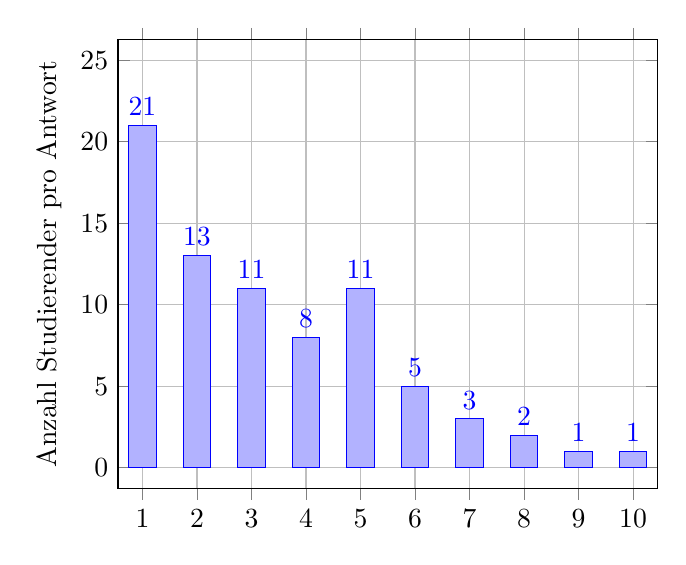
\begin{tikzpicture}
    \begin{axis}[
    	x tick label style={
    		/pgf/number format/1000 sep=},
    	ylabel=Anzahl Studierender pro Antwort,
    	enlargelimits=0.05,
        ymax=25,
        ymin=0,
    	ybar,
        xtick=data,
        xticklabels={1,2,3,4,5,6,7,8,9,10},
        grid=major,
        nodes near coords,
    ]
    \addplot 
    	coordinates {(1,21) (2,13)
    		  (3,11) (4,8) (5,11) (6,5) 
            (7,3) (8,2) (9,1) (10,1)};
    \end{axis}
\end{tikzpicture}